\section{General beskrivelse}

\subsection{Systembeskrivelse}
%Systemet er sammensat af seks dele, som er beskrevet nedenfor. Information omkring delene er fundet i dokumentet: \textit{Scorbot-ER 4u, Users Manual -- 100343-b ER\_4u}
\begin{itemize}

\item Robot \\
Robotten har fem omdrejningsakser, s� den kan man�vrere rundt i systemets omgivelser. Hver del har sin egen motor til at roterer denne del. Ydermere har robotten en klo, der kan gribe fat i elementer og samtidig m�le dem. Figuren nedenfor giver et overblik over robotten.\\

\begin{figure}[h]
\centering
\includegraphics[scale=0.7]{Andet/Robotoversigt.jpg}
\caption{Robotoversigt}
\end{figure}

\item Transportb�nd \\ 
Transportb�ndets opgave er at transportere objekter best�ende af klodser fra en feeder(se billede Figur 2: Systemoversigt) til en position, hvor robotarmen kan f� fat p� klodsen. Dertil er p�monteret en sensor, som stopper b�ndes, n�r klodsen er i den rette position.\\

\item V�gt \\
Der er udleveret en v�gtcelle, hvorudfra der skal konstrueres en fungerende v�gt. V�gten bruges til at veje klodserne, s� materialetypen kan bestemmes. \\

\item STK500-kit \\
STK500-kittet bliver benyttet til AD-konvertering af sp�ndingssignalet der kommer fra v�gten\\

\item USB-Controller og PC \\
For at bruge robotten, skal der g�res brug af en USB-Controlleren, som forbinder disse vha. et 60-pins interface. USB-Controller er koblet til PC'en via et USB-kabel. \\  

\item Database \\
Databasen indeholder data om systemets elementer og logfiler. Det skal v�re muligt at tilg� databasen og �ndre i bestemte elementer.


\end{itemize}

Nedenfor er vist en dom�nemodel, som giver et overblik over systemet.

\begin{figure}[h]
\centering
\includegraphics[scale=0.7]{Domainmodel_Billede.jpg}
\caption{Dom�nemodel}
\end{figure} 

\newpage

\subsubsection{Systemoversigt}
\begin{figure}[h]
\centering
\includegraphics[scale=0.5]{Andet/systemoversigt.jpg} 
\caption{Systemoversigt}
\end{figure}
Ovenst�ende figur giver et overblik over systemet, hvor enhederne ses i sammenh�ng. De forskellige enheder er beskrevet kort i ovenst�ende afsnit, \emph{2.1 Systembeskrivelse}


%\subsubsection{Akt�r kontekst-diagram}

\begin{figure}[h]
\centering
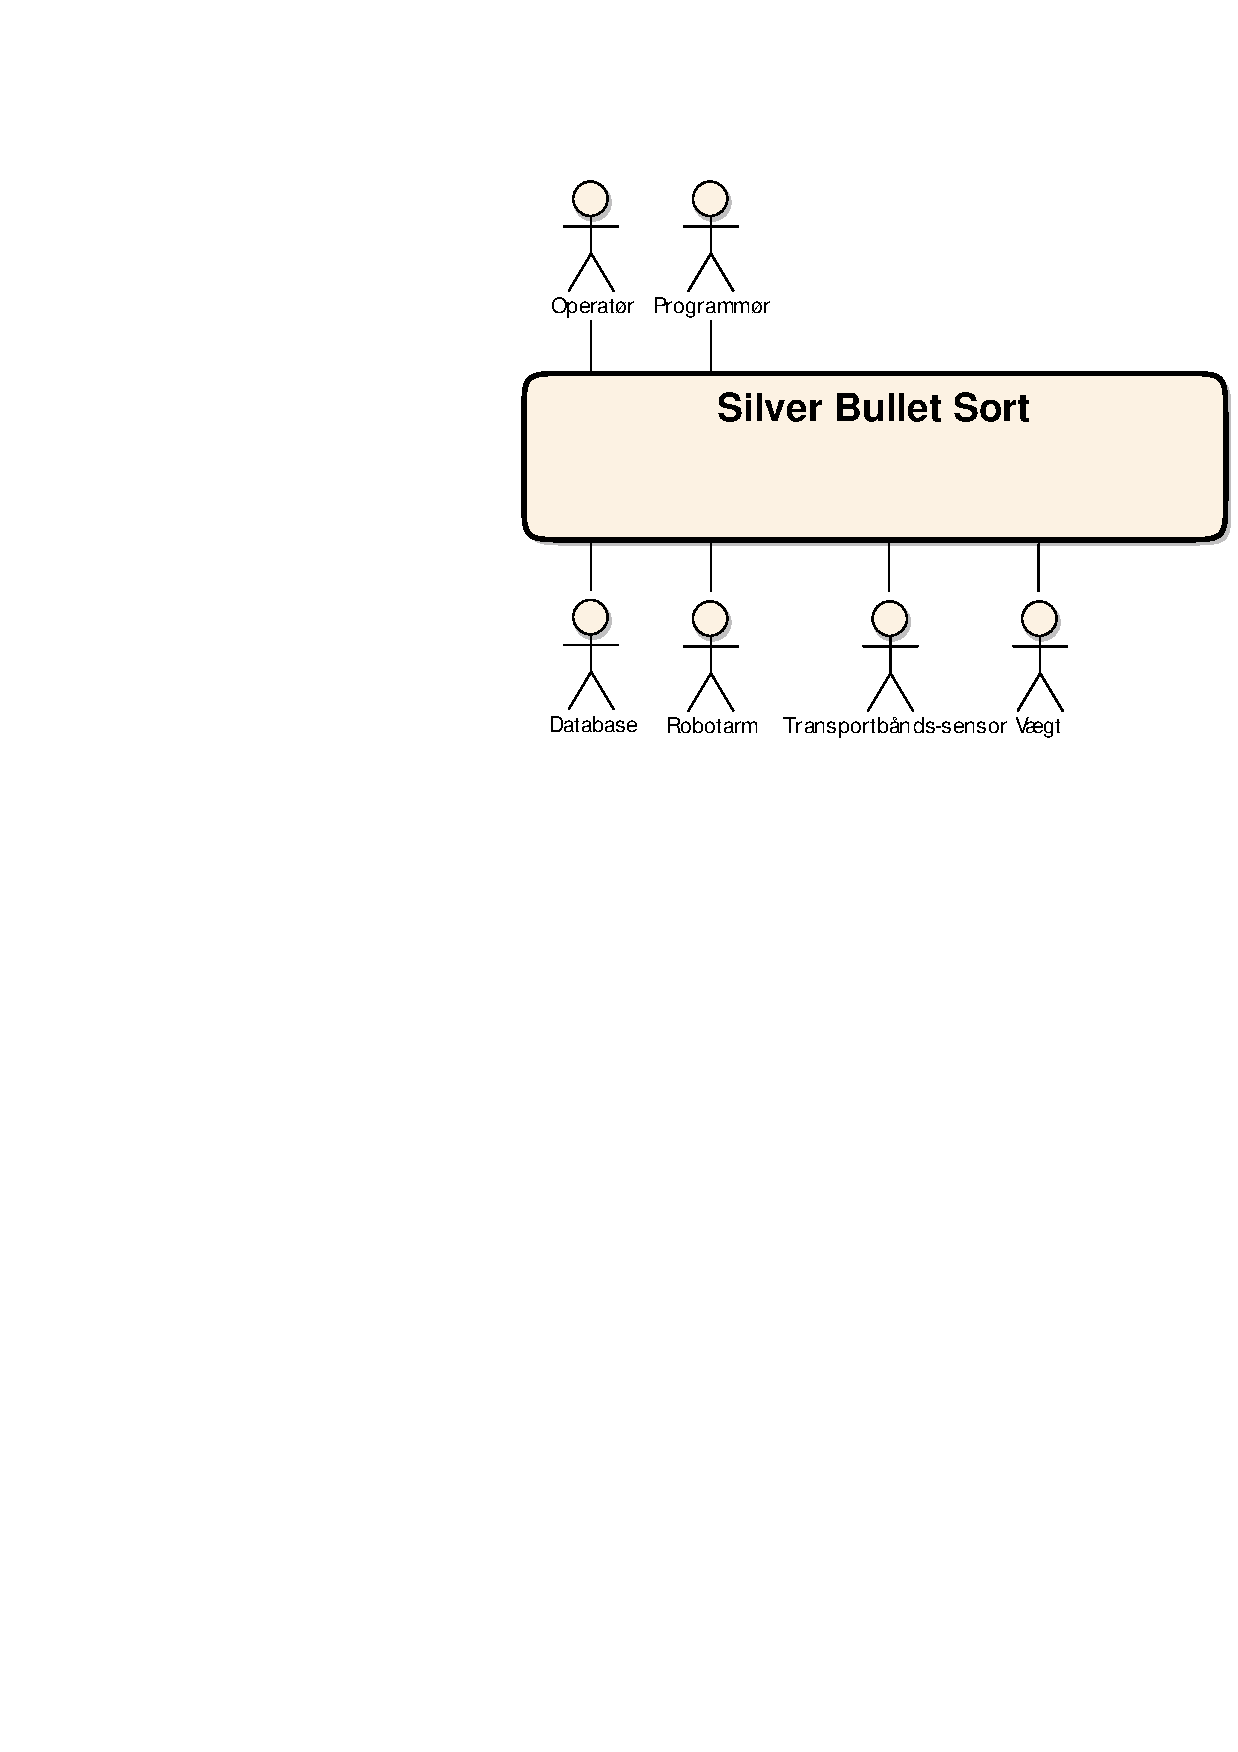
\includegraphics[scale=0.5]{Andet/AktOr-kontekst.jpg}
\caption{Akt�r kontekst-diagram}
\end{figure}

Ovenst�ende figur viser hvilke akt�rer, der interagerer med sorteringssystemet. Videre beskrivelse af disse akt�rer, findes i f�lgende afsnit \emph{2.1.3 Akt�rbeskrivelser}  
\newpage

%\subsubsection{Akt�r beskrivelse}

\underline{\textbf{Prim�re akt�rer:}}\\
\begin{tabular}{lp{10 cm}}

\textbf{Akt�r navn} 				& Operat�r\\
\textbf{Beskrivelse} 				& Denne akt�r starter og stopper systemet. M�let for akt�ren er at f� sorteret klodser, alt efter deres materialetype. \\
\textbf{Antal samtidige akt�rer}	& 1 \\
\\\\
\textbf{Akt�r navn}					&  Programm�r. \\ 
\textbf{Beskrivelse} 				&  Denne akt�rs opgave er at lave brugerdefinerede programmer til systemet.\\ 
\textbf{Antal samtidige akt�rer} 	&  1
\end{tabular}
\\\\
\\\\
\underline{\textbf{Sekund�re akt�rer}}
\\
\begin{tabular}{lp{10 cm}}

\textbf{Akt�r navn} 				& V�gt\\
\textbf{Beskrivelse} 				& Denne akt�r vejer et objekt, s� systemet kan bestemme dets materialetype.  \\
\textbf{Antal samtidige akt�rer}	& 1 \\
\\\\
\textbf{Akt�r navn}					& Transportb�ndssensor \\
\textbf{Beskrivelse}				& Denne akt�r registrerer, hvorn�r et objekt er klar til at blive samlet op af robotten.  \\
\textbf{Antal samtidige akt�rer}	& 1 \\
\\\\
\textbf{Akt�r navn} 				&  Robotarm.\\ 
\textbf{Beskrivelse} 				&  Denne akt�rs opgave er at flytte og m�le forskellige typer klodser.\\ 
\textbf{Antal samtidige akt�rer} 	&  1 \\ 
\\\\
\textbf{Akt�r navn} 				&  Database. \\ 
\textbf{Beskrivelse} 				&  Databasen indeholder logfiler for systemets data for de enkelte klodser, samt informationer om robotten og systemets status. Ligeledes indeholder databasen programmerne, som programm�ren har lavet.\\ 
\textbf{Antal samtidige akt�rer} 	&  1
\end{tabular} 
